\section{Capitolo 4}



	\subsection{Esercizio 4.1}
	
Scrivere una function Matlab che implementi il calcolo del polinomio interpolante di grado $n$ in forma di Lagrange. La forma della function deve essere del tipo \texttt{ y = lagrange( xi, fi, x ) }.
\PP
La base di Lagrange è così definita:
\begin{equation}
	L_{kn} := \prod_{j=0,j\neq{k}}^n\frac{x-x_j}{x_k-x_j}
\end{equation}
La forma di Lagrange del polinomio interpolante è:
\begin{equation}\label{lagrange_equation}
	\sum_{k=0}^n f(x_k) L_{kn}(x)
\end{equation}
La function Matlab che implementa la \ref{lagrange_equation} è:
\lstinputlisting{./capitolo_4/lagrange.m}
Costi: dati $n$ numero di ascisse di interpolazione e $m$ numero di punti da calcolare l'occupazione di memoria è pari al vettore $\mathbf{y}$ in output che ha dimensione $m$ mentre il numero di flops è $2mn(2n+1)$.



	\subsection {Esercizio 4.2}
	
Scrivere una function Matlab che implementi il calcolo del polinomio interpolante di grado $n$ in forma di Newton. La forma della function deve essere del tipo \texttt{ y = newton( xi, fi, x ) }
\PP
La base di Newton è così definita: 
\begin{empheq}[left=\empheqlbrace]{align}
	& \omega_0(x):=1 \\
	& \omega_1(x):=x-x_0 \\
	& ... \\
	& \omega_{i+1}(x):=(x-x_i)\omega_i(x)
\end{empheq}
La forma di Newton del polinomio interpolante rispetto alla base di Newton è:
\begin{equation} \label{newton_equation}
	\sum_{k=0}^n f[x_0, ... , x_k]\omega_k(x)
\end{equation} 
La function matlab che implementa \ref{newton_equation} è:
\lstinputlisting{./capitolo_4/newton_interpolation.m}



	\subsection {Esercizio 4.3}
	
Scrivere una function Matlab che implementi il calcolo del polinomio interpolante di Hermite. La forma della function deve essere del tipo \texttt{ y = hermite( xi, fi, f1i, x ) }
\PP
Il polinomio interpolante di Hermite richiede un numero pari di ascisse distribuite come segue: 
\begin{equation}
	a <= x_0 < x_{\frac{1}{2}} < x_{1+\frac{1}{2}} < ... < x_n < x_{n+\frac{1}{2}} <= b
\end{equation}
con $\lim{x_{i+\frac{1}{2}} = x_i}$ si ha che $x_0 = x_1$, $x_2=x_3$, etc. Pertanto $f[x_i, x_1]:=f[x_i, x_i]:=f^{(1)}(x_i)$ e l'algoritmo delle differenze divise verrà modificato in modo che al primo passo quando bisogna calcolare $f[x_i, x_i]$ si utilizza il valore della derivata prima che verrà passato come parametro alla funzione.

La function Matlab che implementa il polinomio interpolante di Hermite è:
\lstinputlisting{./capitolo_4/hermite.m}


	\pagebreak
	\subsection {Esercizio 4.4}
	
Utilizzare le functions degli esercizi precedenti per disegnare l'approssimazione della funzione $sin(x)$  nell'intervallo $[0, 2\pi]$, utilizzando le ascisse di interpolazione $x_{i}=i\pi, i=0,1,2$.
\PP
Il codice seguente richiama le funzioni definite in precedenza e disegna un grafico con le funzioni $sin(x)$ ed i polinomi interpolanti.
\lstinputlisting{./capitolo_4/sin_interpolation.m}
Il risultato è stato riportato in figura \ref{sin_interpolation}.

\begin{figure}[h]\label{sin_interpolation}
    \centering
    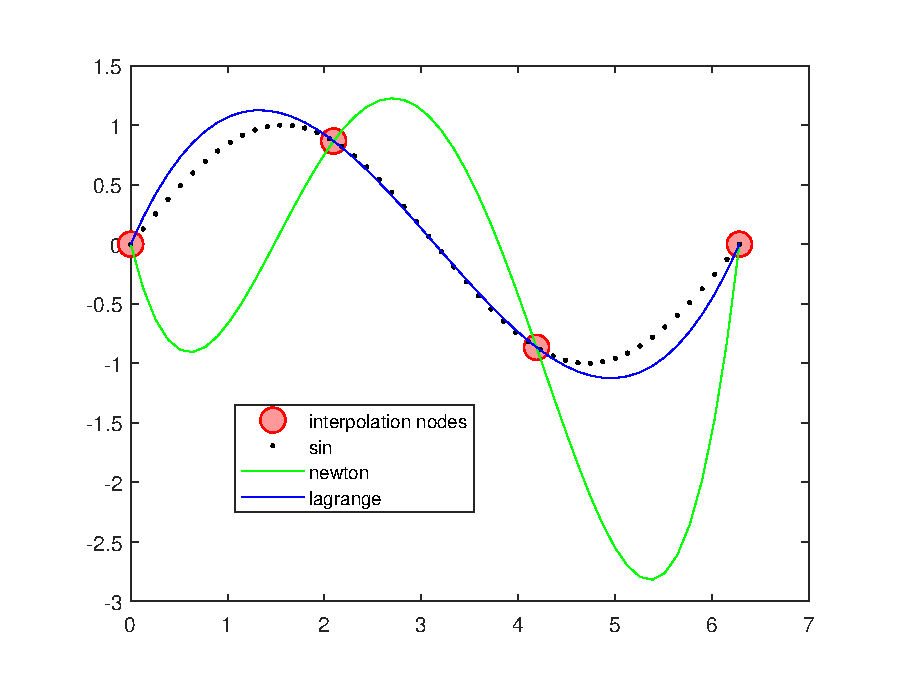
\includegraphics[scale=0.8]{./capitolo_4/sin_interpolation}
    \caption{Interpolazione usando forma di Lagrange e di Newton}
\end{figure} 



	\subsection {Esercizio 4.5}
	
Scrivere una function Matlab che implementi la \texttt { spline } cubica interpolante (naturale o \textit{not-a-knot}, come specificato in ingresso) delle coppie di dati assegnate. La forma della function deve essere del tipo: \texttt { y = spline3( xi, fi, x, tipo ) }.
\PP
Formule per il calcolo della spline cubica:
\begin{equation*}
	\begin{split}
		\forall x \in \lbrack x_{i-1}, x_i \rbrack & : \\
		s_3(x_i) & = \frac{h_i^2}{6}m_i + q_i h_i +r_i \\
		s_3(x_{i-1}) & = \frac{h_i^2}{6}m_{i-1} + r_i \\
		h_i & = x_i - x_{i-1} \\
		q_i & = \frac{f_i - f_{i-1}}{h_i} - \frac{h_i}{6}(m_i -m_{i-1})\\ 
		r_i &= f_{i-1}  - \frac{h_i^2}{6}m_{i-1} \\
		\forall i = 1, 2 \cdots n-1 & : \\
		\varphi_i & = \frac{h_i}{h_i+h_{i+1}} \\
		\xi_i & = \frac{h_{i+1}}{h_i+h_{i+1}} 
	\end{split}
\end{equation*}

I valori $m_i$ sono la soluzione dei seguenti sistemi lineari tridiagonali,
per la spline \textit{naturale}:
\[
	\begin{pmatrix}
		2 		& \xi_1 	& 			& 		& 	\\
		\varphi_2 	& 2			& \xi_2	& 		& 	\\
				& ...			& ...			& ... 	& 	\\
				& 			& ...			& ... 	& \xi_{n-2}	\\
				& 			& 			& \varphi_{n-1} 	& 2	\\
	\end{pmatrix}
	\begin{pmatrix}
		m_1 \\
		m_2 \\
		... \\
		... \\
		m_{n-1}
	\end{pmatrix}
	= 6
	\begin{pmatrix}
		f[x_0, x_1, x_2] \\
		f[x_1, x_2, x_3] \\
		... \\
		... \\
		f[x_{n-2}, x_{n-1}, x_n] \\
	\end{pmatrix}
\]
mentre per la spline \textit{not-a-knot}:
\[
	\begin{smallmatrix}
		1 & 0 & & & & & \\
		\varphi_1 & 2-\varphi_1 & \xi_1 - \varphi_1 & & & & \\
		 & \varphi_2 & 2 & \xi_2 & & & \\
		 & & ... & ... & ... & & \\
		 & & & \varphi_{n-2} & 2 & \xi_{n-2} & \\
		 & & & &  \varphi_{n-1} - \xi_{n-1} & 2-\xi_{n-1} & \xi_{n-1} \\
		 & & & & & 0 & 1 \\
	\end{smallmatrix}
	\begin{smallmatrix}
		m_0+m_1+m_2 \\
		m_1 \\
		... \\
		... \\
		... \\
		m_{n-1}\\
		m_n+m_{n-1}+m_{n-2} \\		
	\end{smallmatrix}
	= 6
	\begin{smallmatrix}
		f[x_0, x_1, x_2] \\
		f[x_0, x_1, x_2] \\
		... \\
		... \\
		... \\
		f[x_{n-2}, x_{n-1}, x_n] \\
		f[x_{n-2}, x_{n-1}, x_n] \\
	\end{smallmatrix}
\]

questo porta al seguente codice per calcolare la spline:
\lstinputlisting{./capitolo_4/my_spline/spline3.m}


	\subsection {Esercizio 4.6}
	
Scrivere una function Matlab che implementi il calcolo delle ascisse di Chebyshev per il polinomio interpolante di grado $n$, su un generico intervallo $[a,b]$. La function deve essere del tipo: \texttt { xi = ceby( n, a, b ) }.
\PP
La function per le ascisse di Chebyshev è:
\lstinputlisting{./capitolo_4/chebyshev_abscissas.m}



	\subsection {Esercizio 4.7}
	
Utilizzare le function degli Esercizi 4.1 e 4.6 per graficare l'approssimazione della funzione di Runge sull'intervallo $[-6,6]$ per $n= 2,4, ... ,40$. Stimare, numericamente, l'errore commesso in funzione del grado $n$ del polinomio interpolante.
\PP
Lo script:
\lstinputlisting{./capitolo_4/exercise_4_7.m}
esegue la function \lstinline{lagrange} con il risultato della function \lstinline{chebyshev_abscissas}, il risultato è stato riportato in figura \ref{4_7_lagrange_interpolation}.\\
\begin{figure}[h!]\label{4_7_lagrange_interpolation}
    \centering
    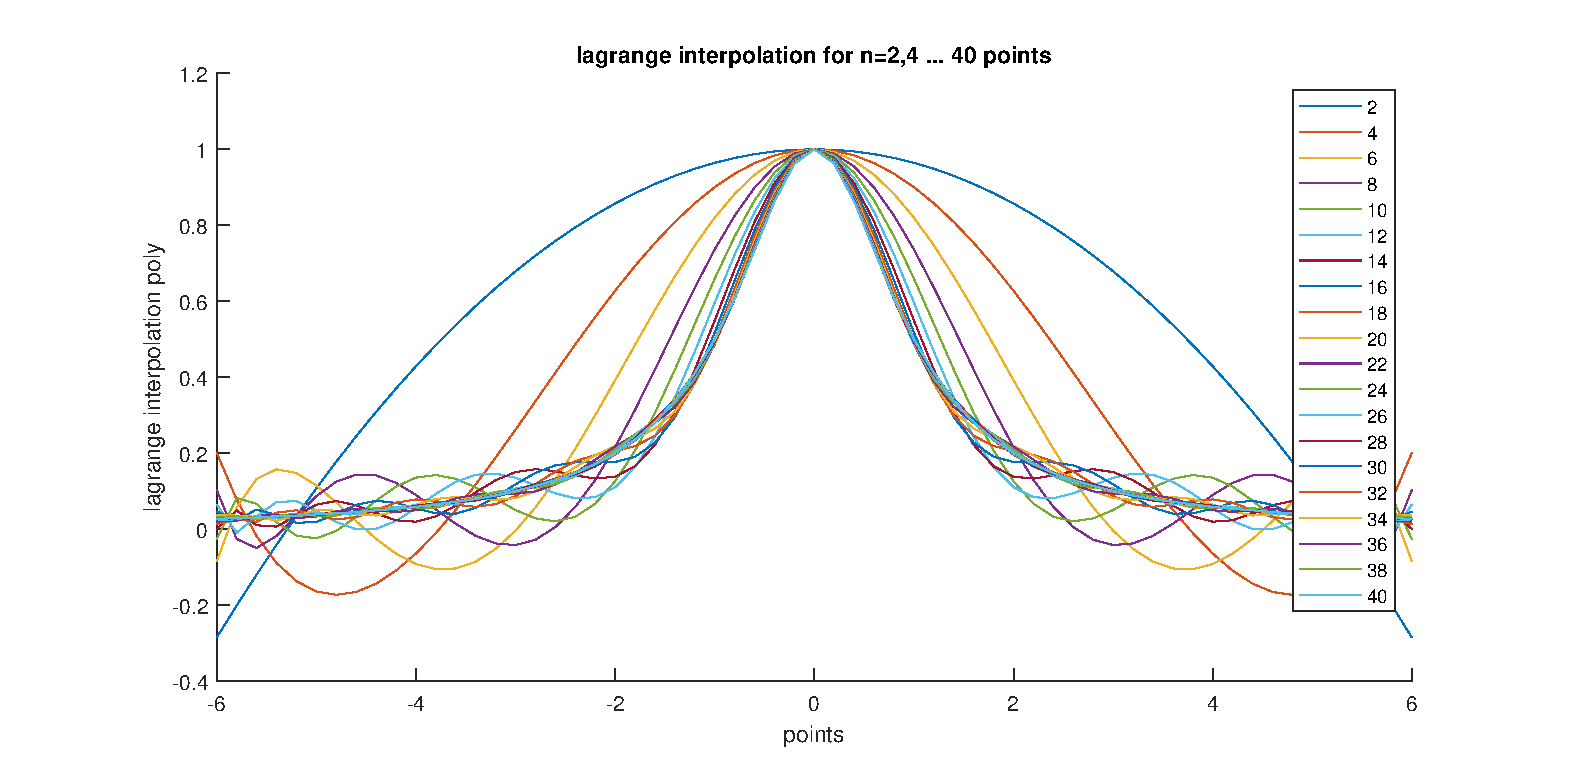
\includegraphics[scale=0.5]{./capitolo_4/exercise_4_7}
    \caption{Interpolazione con ascisse di Chebyshev usando il polinomio in forma di Lagrange per funzione di Runge}
\end{figure}
\PP
L'errore, in relazione al grado $n$ del polinomio, è quantificabile in $\norm{e} <= \frac{\norm{f^{n+1}}}{(n+1)!2^n}$:
\begin{tabular}{ | c | r }
\textbf{n} & \multicolumn{1}{c}{$\mathbf{\norm{e}}$} \\
\hline
2  &   0.18557  \\
4  &  0.051465  \\
6  &  0.013356  \\
8  & 0.0029532  \\
10 & 0.00053885 \\
\end{tabular}
\begin{tabular}{ | c | r }
\textbf{n} & \multicolumn{1}{c}{$\mathbf{\norm{e}}$} \\
\hline
12 & 7.0571e-05 \\
14 & 3.6605e-06 \\
16 & 4.2884e-06 \\
18 &   1.86e-06 \\
20 & 5.7764e-07 \\
\end{tabular}
\begin{tabular}{ | c | r }
\textbf{n} & \multicolumn{1}{c}{$\mathbf{\norm{e}}$} \\
\hline
22 & 1.4887e-07 \\
24 & 3.2687e-08 \\
26 & 5.9039e-09 \\
28 & 7.3124e-10 \\
30 & 3.2957e-11 \\
\end{tabular}
\begin{tabular}{ | c | r }
\textbf{n} & \multicolumn{1}{c}{$\mathbf{\norm{e}}$} \\
\hline
32 & 4.9639e-11 \\
34 & 2.1068e-11 \\
36 & 6.4812e-12 \\
38 & 1.6589e-12 \\
40 & 3.6167e-13
\end{tabular}



	\subsection {Esercizio 4.8}
	
Relativamente al precedente esercizio, stimare numericamente, la crescita della costante di Lebesgue.
\PP
Considerando che la costante di Lebesgue nel caso delle ascisse di Chebyshev è $\Lambda_n \approx \frac{2}{\pi}\log{n} $ si ha la seguente tabella relativa agli $n=2,4,6 ... 40$:\\
\begin{tabular}{ | c | r | r }
\textbf{n} & \multicolumn{1}{c}{$\mathbf{\Lambda_n}$} & \multicolumn{1}{c}{\textbf{\%}}\\
\hline
      2   &  0.44127  &     100  \\
      4   &  0.88254  &     100  \\
      6   &   1.1407  &  29.2  \\
      8   &   1.3238  &  16.0  \\
     10   &   1.4659  &  10.7  \\
\end{tabular}
\begin{tabular}{ | c | r | r }
\textbf{n} & \multicolumn{1}{c}{$\mathbf{\Lambda_n}$} & \multicolumn{1}{c}{\textbf{\%}}\\
\hline
     12   &   1.5819  &  7.9  \\
     14   &   1.6801  &  6.2  \\
     16   &   1.7651  &  5.0  \\
     18   &   1.8401  &  4.2  \\
     20   &   1.9071  &  3.6  \\
\end{tabular}
\begin{tabular}{ | c | r | r }
\textbf{n} & \multicolumn{1}{c}{$\mathbf{\Lambda_n}$} & \multicolumn{1}{c}{\textbf{\%}}\\
\hline
     22   &   1.9678  &  3.1  \\
     24   &   2.0232  &   2.8  \\
     26   &   2.0742  &  2.5  \\
     28   &   2.1213  &  2.3  \\
     30   &   2.1653  &  2.1  \\
\end{tabular}
\begin{tabular}{ | c | r | r }
\textbf{n} & \multicolumn{1}{c}{$\mathbf{\Lambda_n}$} & \multicolumn{1}{c}{\textbf{\%}}\\
\hline
     32   &   2.2064  &  1.9  \\
     34   &    2.245  &  1.7  \\
     36   &   2.2813  &  1.6  \\
     38   &   2.3158  &  1.5  \\
     40   &   2.3484  &  1.4  \\
\end{tabular}



	\subsection {Esercizio 4.9}
	
Utilizzare la function dell'esercizio 4.1 per approssimare la funzione di Runge sull'intervallo $[-6,6]$, su una partizione uniforme di $n+1$ ascisse, $n= 2,4, ... ,40$. Stimare le corrispondenti costanti di Lebesgue.
\PP
Lo script che usa e graficizza il risultato della function \lstinline{lagrange} è il seguente:
\lstinputlisting{./capitolo_4/exercise_4_9.m}
il valore $n$ è stato ristretto a $n=12$ perché oltre la funzione interpolante assume valori elevatissimi in corrispondenza degli estremi ed il grafico non avrebbe nessuna valenza informativa. Già con $n=12$ si verifica che verso gli estremi la funzione assume valori molto elevati e questo è dovuto alla crescita rapida della costante di Lebesgue. 
Il grafico è stato riportato in figura \ref{4_9_lagrange_interpolation}.\\
\begin{figure}[h!]\label{4_9_lagrange_interpolation}
    \centering
    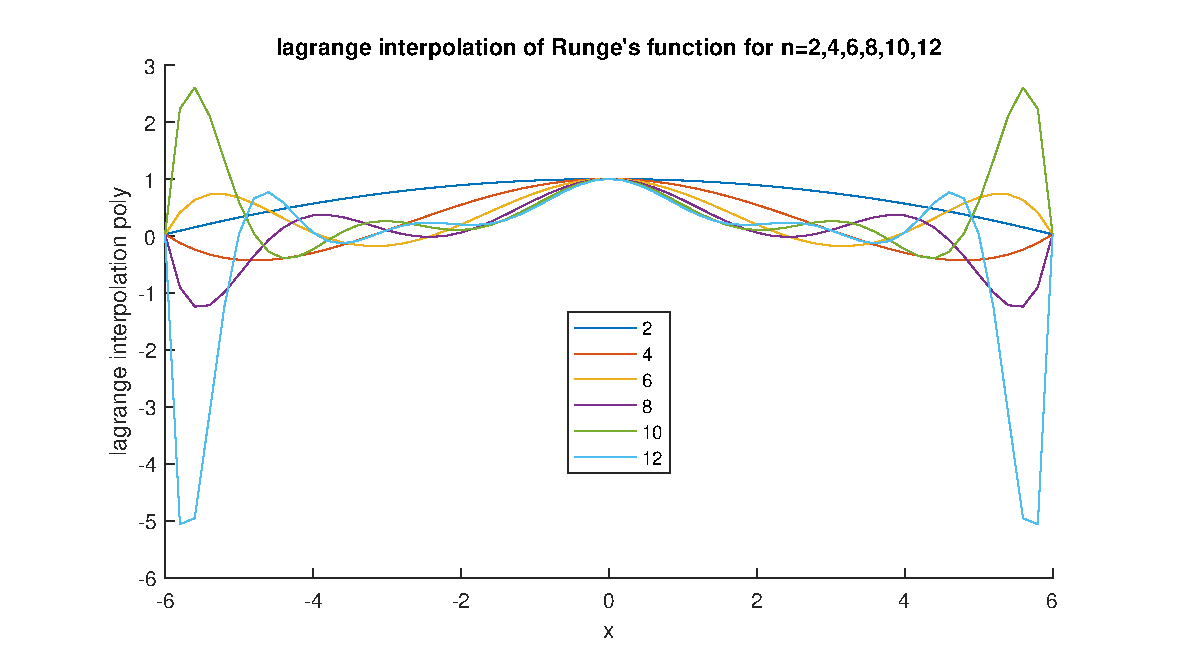
\includegraphics[scale=0.5]{./capitolo_4/exercise_4_9}
    \caption{Interpolazione con ascisse equidistanti usando il polinomio in forma di Lagrange per funzione di Runge}
\end{figure}
Usando questo script:
\lstinputlisting{./capitolo_4/exercise_4_9_lebesgue.m}
anch'esso ristretto a $n=12$ si osserva che la costante aumenta molto rapidamente verso gli estremi all'aumentare di $n$.
Il risultato grafico è riportato in figura \ref{fig:4_9_lebesgue}.\\
\begin{figure}[h!]
    \centering
    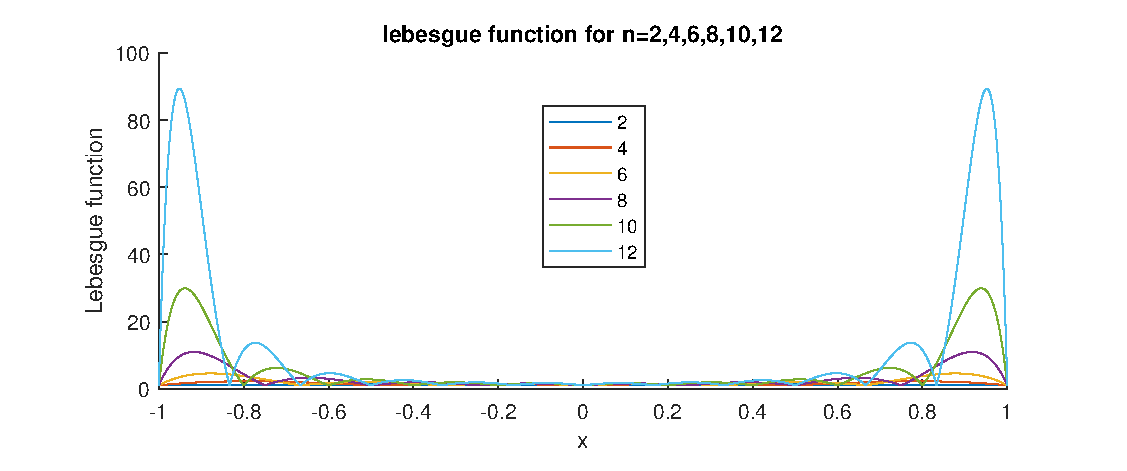
\includegraphics[scale=0.7]{./capitolo_4/exercise_4_9_lebesgue}
    \label{fig:4_9_lebesgue}
    \caption{Valori della funzione di Lebesgue per n= 2,4,6,...,12}
\end{figure}



	\subsection {Esercizio 4.10}

Stimare, nel senso dei minimi quadrati, posizione, velocità iniziale ed accelerazione relative a un moto rettilineao uniformemente accelerato per cui sono note le seguenti misurazioni delle coppie (tempo, spazio): (1, 2.9), (1, 3.1), (2, 6.9), (2, 7.1), (3, 12.9), (3, 13.1), (4, 20.9), (4, 21.1), (5, 30.9), (5, 31.1).
\PP
La formula del moto uniformemente accelerato è:
\begin{equation*}
	x(t) = x_0 + v_0t +\frac{1}/{2}at^2
\end{equation*}
che è un polinomio di grado $n=2$ quindi abbiamo bisogno di almeno $n+1$ ascisse distinte, in questo caso ne abbiamo $5$ pertanto stimare $x_0, \quad v_0, \quad a_0$ equivale a risolvere il seguente sistema sovradeterminato:

\[
	A = 
	\begin{pmatrix}
		1^0 & 1^1 & 1^2 \\
		1^0 & 1^1 & 1^2 \\
		2^0 & 2^1 & 2^2 \\
		2^0 & 2^1 & 2^2 \\
		3^0 & 3^1 & 3^2 \\
		3^0 & 3^1 & 3^2 \\
        	4^0 & 4^1 & 4^2 \\
		4^0 & 4^1 & 4^2 \\
        	5^0 & 5^1 & 5^2 \\
		5^0 & 5^1 & 5^2 \\
	\end{pmatrix}
	\begin{pmatrix}
		x_0 \\
		v_0 \\
		a_0 \\
	\end{pmatrix}
	=
	\begin{pmatrix}
		2.9 \\
		3.1 \\
		6.9 \\
		7.1 \\
		12.9 \\
		13.1 \\
		20.9 \\
		21.1 \\
		30.9 \\
		31.1 \\
	\end{pmatrix}
\]

Usando lo script:

\lstinputlisting{./capitolo_4/exercise_4_10.m}
che risolve il sistema tramite una fattorizzazione $QR$ della matrice $A$ si ottiengono i risultati:
\[
		\mathbf{x} = \begin{pmatrix} x_0 \\ v_0 \\ a_0 \end{pmatrix}  = \begin{pmatrix} 1 \\ 1 \\ 1 \end{pmatrix} 
		, \qquad
		r \equiv A\mathbf{x} - \mathbf{b} = \begin{pmatrix} 0.1 \\ -0.1 \\ 0.1 \\ -0.1 \\ 0.1 \\ -0.1 \\ 0.1 \\ -0.1 \\ 0.1 \\ -0.1 \\ \end{pmatrix} 
\]
